\documentclass[hyperref={bookmarks=false},aspectratio=169]{beamer}
\usepackage[utf8]{inputenc}
\usepackage{amsmath}
\usepackage{graphicx}
\usepackage{subcaption}
\usepackage{array}
% ---------------  Define theme and color scheme  -----------------
\usetheme[minimal]{Caltech}  % 3 options: minimal, sidebarleft, sidebarright

%\setbeamertemplate{footline}[frame number]

% ------------  Information on the title page  --------------------
\title[A Swampland Constraint on Gravitational Collapse]
{\bfseries{A Swampland Constraint on Gravitational Collapse}}

\subtitle{Master's thesis by Himanshu Chaudhary}

\author[Himanshu Chaudhary]
{\textbf{Advisor}: Chethan Krishnan\inst{1}
\and \\
\textbf{Committe members}:
Prasad Hegde\inst{1} \and Sachindeo Vaidya\inst{1}
} 
% {Mischief\inst{1} \and Managed\inst{2}}

\institute[IISc]
{
  \inst{1}
  Center for High Energy Physics\\
  Indian Institute of Science
  % \and
  % \inst{2}
  % Department of Student Pranks\\
  % California Institute of Technology
}

\date[IISc, 2020]
{1st July, 2020}
% {International Conference on University Pranks\\April 1st, 2014}
%------------------------------------------------------------

%------------------------------------------------------------
%The next block of commands puts the table of contents at the 
%beginning of each section and highlights the current section:

% \AtBeginSection[]
% {
%   \begin{frame}
%     \frametitle{Table of Contents}
%     \tableofcontents[currentsection]
%   \end{frame}
% }
%------------------------------------------------------------


\begin{document}

\frame{\titlepage}  % Creates title page

% %---------   table of contents after title page  ------------
% \begin{frame}
%   \frametitle{Table of Contents}
%   % \tableofcontents
% \end{frame}
% %---------------------------------------------------------


\section{Caltech student traditions}

%---------------------------------------------------------
%Changing visivility of the text
\begin{frame}
  \frametitle{Introduction}
  Gravitational collapse of a scalar field is a well studied phenomenon but, most of
  these studies are narrowly focussed on studying the field behavior close to criticality
  and its implications. In this thesis we take a broader perspective and study the
  gravitational collapse in the context of the Swampland bounds and Effective field
  theories. We are particularly interested in the Swampland distance bound, according
  to which a classical solution where scalar fields move by an O(1) range (in Plank
  units) signals the breakdown of Effective Field Theory.


  % \begin{itemize}
  %   \item<1-> A claim was once made that the shattering of a pumpkin frozen in liquid nitrogen and dropped from a sufficient height would produce a triboluminescent spark.
  %   \item<2-> This yearly event involves a crowd of observers, who try to spot the elusive spark.
  %   \item<3-> The title of the event is an oblique reference to the famous Millikan oil-drop experiment which measured $e$, the elemental unit of electrical charge.
  % \end{itemize}

\end{frame}





\begin{frame}
  \frametitle{Effective field theories}

  \begin{itemize}
    \item What is an EFT (just in the context of QFT)?
    \item Example of an EFT
    \item EFT are supposed to hold at the Horizon
  \end{itemize}


\end{frame}


\begin{frame}
  \frametitle{Swampland Distance Conjecture}
  \begin{itemize}
    \item Define what is landscape
    \item Define what is Swampland
  \end{itemize}

\end{frame}


\begin{frame}
  \frametitle{Swampland Distance Conjecture}
  \begin{itemize}
    \item What are Swampland bounds
    \item Do mention that are nothing but ideas
    \item Swampland distance bound
          % \item 
  \end{itemize}

\end{frame}

\begin{frame}
  \frametitle{Gravitational Collapse}

  \begin{itemize}
    \item Describe collapse of a minimally coupled scalar field.
    \item Talk about the known results
    \item Talk about our results
  \end{itemize}

\end{frame}


\begin{frame}
  \frametitle{Scalar gravitational collapse}
  % \begin{itemize}
  %   \item Write the action
  %   \item The metric
  %   \item The
  % \end{itemize}
  \begin{equation*}
    S=\frac{1}{8 \pi G} \int d^{4} x \sqrt{-g}\left(\frac{1}{2} R-\frac{1}{2} \partial_{\mu} \phi \partial^{\mu} \phi\right)
  \end{equation*}
  \begin{equation*}
    ds^2=e^{-2 \sigma(t, x)}\left(-d t^{2}+d x^{2}\right)+r^{2}(t, x) d \Omega^{2}
  \end{equation*}
  \begin{equation*}
    r\left(-r_{, t t}+r_{, x x}\right)-r_{, t}^{2}+r_{x}^{2}=e^{-2 \sigma}
  \end{equation*}

  \begin{equation*}
    -\sigma_{, t t}+\sigma_{,x x}+\frac{r_{, t t}-r_{,x x}}{r}+4 \pi\left(\psi_{, t}^{2}-\psi_{, x}^{2}\right)=0
  \end{equation*}

  \begin{equation*}
    -\psi_{, t t}+\psi_{,x x}+\frac{2}{r}\left(-r_{, t} \psi_{, t}+r_{, x} \psi_{, x}\right)=0
  \end{equation*}


\end{frame}

\begin{frame}
  \frametitle{Constraint equations}
  \begin{equation}
    r_{, t x}+r_{, t} \sigma_{, x}+r_{, x} \sigma_{, t}+4 \pi r \psi_{, t} \psi_{, x}=0
    \label{eqn:constraint_1}
  \end{equation}

  \begin{equation}
    r_{, t t}+r_{, x x}+2 r_{, t} \sigma_{, t}+2 r_{, x} \sigma_{, x}+4 \pi r\left(\psi_{, t}^{2}+\psi_{, x}^{2}\right)=0
    \label{eqn:constraint_2}
  \end{equation}

  They will be used to generate inital conditions

  They will be used to check out results



\end{frame}

\begin{frame}
  \frametitle{Introducing Mister sharpe mass}
  \begin{equation*}
    g^{\mu \nu} r_{, \mu} r_{, \nu}=e^{2 \sigma}\left(-r_{, t}^{2}+r_{, x}^{2}\right) \equiv 1-\frac{2 m}{r}
  \end{equation*}

  Helps with the stability


\end{frame}


\begin{frame}
  \frametitle{Final equations to solve}

  \begin{equation}
    -\psi_{, t t}+\psi_{, x x}+\frac{2}{r}\left(-r_{, t} \psi_{, t}+r_{, x} \psi_{, x}\right)=0
    \label{eqn:psi}
  \end{equation}

  \begin{equation}
    -r_{, t t}+r_{, x x}-e^{-2 \sigma} \cdot \frac{2 m}{r^{2}}=0
    \label{eqn:r}
  \end{equation}

  \begin{equation}
    -\sigma_{, t t}+\sigma_{, x x}-e^{-2 \sigma} \cdot \frac{2 m}{r^{3}}+4 \pi\left(\psi_{, t}^{2}-\psi_{, x}^{2}\right)=0
    \label{eqn:sigma}
  \end{equation}

  \begin{equation}
    m_{, t}=4 \pi r^{2} \cdot e^{2 \sigma}\left[-\frac{1}{2} r_{, t}\left(\psi_{, t}^{2}+\psi_{, x}^{2}\right)+r_{, x} \psi_{, t} \psi_{, x}\right]
    \label{eqn:m_t}
  \end{equation}


\end{frame}

\begin{frame}
  \frametitle{Boundary conditions}
  To get the boundary conditions at the origin we will use regularity arguments.
  Observe that $r$ is always set to $0$ at $x=0$, this is done to prevent formation of any kind of cusp at the origin, which give us $r_{,t}(t,0) = 0$ and $r_{,tt}(t,0)=0$.
  Now, to ensure that the term $\frac{2}{r}\left(-r_{, t} \psi_{, t}+r_{, x} \psi_{, x}\right)$ from the equation \ref{eqn:psi} is regular at the origin we need that $r_{, x} \psi_{, x} = 0$ because $r_{,t}(t,0)$ is already $0$, therefore we have that $\psi_{,x}(t,0) = 0$. Looking at the equation \ref{eqn:m_definition} we can see that we need $m(t,0) = 0 $ to keep the term $\frac{2 m}{r}$ regular. Similarly from the equation \ref{eqn:r} we get that $r_{,xx}=0$. Finally, at the origin the equation \ref{eqn:constraint_2} becomes $r_{,x} \sigma_{,x} = 0$ which gives us $\sigma_{,x}(t,0) = 0$.

\end{frame}


\begin{frame}
  \frametitle{Boundary conditions}

  One can see that not all of these boundary conditions are independent. To evolve the initial data we will use the following four boundary conditions at the origin,

  \begin{eqnarray*}
    r(t,0) = 0 \\
    m(t,0) =0 \\
    \psi_{,x}(t,0) = 0\\
    \sigma_{,x}(t,0) = 0
  \end{eqnarray*}
\end{frame}


\begin{frame}
  \frametitle{Inital conditions}

  \begin{equation}
    r_{, t}=\sigma_{, t}=\phi_{, t}=\psi_{, t}=0 \quad \text { at } t=0
    \label{eqn:time_symmetric_boundary_conditinons}
  \end{equation}

  \begin{equation}
    r_{, x x}=e^{-2 \sigma} \cdot \frac{2 m}{r^{2}}
    \label{eqn:r_chap3}
  \end{equation}


  \begin{equation}
    \sigma_{, x}= -2 \pi \cdot  \frac{\psi_{, x}^{2} \cdot r}{r_{,x}}- e^{-2 \sigma} \cdot \frac{ m}{r^{2}r_{, x}}
    \label{eqn:sigma_chap3}
  \end{equation}

  \begin{equation}
    m_{, x}=4 \pi r^{2} \cdot e^{2 \sigma}\left[\frac{1}{2} r_{, x} \cdot \psi_{, x}^{2} \right]
  \end{equation}


\end{frame}


\begin{frame}
  \frametitle{Boundary Condtitinos for the inital conditions}
  \begin{eqnarray*}
    r(0 ,0) = 0  \\
    r_{,x}(0 ,0) = 1  \\
    \sigma(0 ,0) = 1  \\
    m(0 ,0) = 1
  \end{eqnarray*}
\end{frame}

\begin{frame}
  \frametitle{Floating point errors}
  What are floating point errors?
  \begin{table}[hbt!]
    \centering
    \begin{tabular}{||m{2cm} | m{3.0cm} | m{1.5cm} | m{4.5cm}||}
      \hline
      Float type & Largest Number that can be stored* & Precision & How is $\frac{1}{3}$ internally stored \\ [0.5ex]
      \hline\hline

      Float32    & 3.40e+38                           & 6         & 0.33333334                             \\

      Float64    & 1.79e+308                          & 15        & 0.3333333333333333                     \\

      Float128   & 3.36e+4932                         & 18        & 0.33333333333333333334                 \\ [1ex]
      \hline
    \end{tabular}
    \caption{This table shows the largest number that can be represented by a particular type of float (* rounded off to two decimal places). Precision denotes the number of significant decimal digits that can be represented by a float type.}
    \label{table:floats}
  \end{table}
\end{frame}

\begin{frame}
  \frametitle{Finite difference: First Order}
  \begin{columns}
    \column{0.3\textwidth}
    \begin{equation*}
      y'(x_0)  \approx \frac{y(x_0 + h) - y(x_0)}{h}
      \label{eq:1d_1o_error}
    \end{equation*}
    \column{0.7\textwidth}
    \begin{figure}[hbt!]
      \centering
      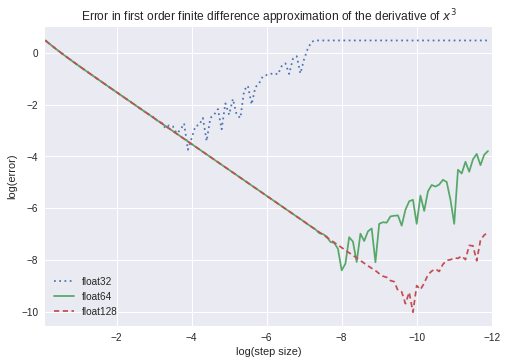
\includegraphics[width=\textwidth]{images/x^3_error_order1.png}
      % \caption[Error in the approximation of the first derivative of $x^3$ by first order finite difference methods.]{This plot show error of using first order finite difference to approximate the derivative of $x^3$ vs the step size. Observe that the error falls almost linearly until the floating point errors start to dominate, after which it starts to grow erratically. Also, observe that for reasonable step sizes the error falls with a slope of 1, which is why such approximations are called to be of first order. }\label{fig:x^3_error_order1}
      \index{figures}


    \end{figure}

  \end{columns}
\end{frame}


\begin{frame}
  \frametitle{Finite difference: Second order}
  \begin{columns}
    \column{0.35\textwidth}
    \begin{equation*}
      y'(x_0)  \approx \frac{y(x_0 + h) - y(x_0 - h)}{2 \times h}
      \label{eq:d_second_order}
    \end{equation*}
    \column{0.7\textwidth}
    \begin{figure}[hbt!]
      \centering
      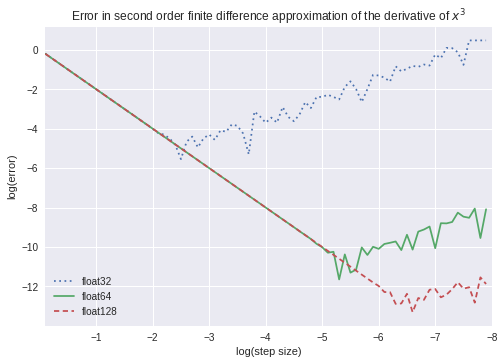
\includegraphics[width=\textwidth]{images/x^3_error_order2.png}
      % \caption[Error in the approximation of the first derivative of $x^3$ by first order finite difference methods.]{This plot show error of using first order finite difference to approximate the derivative of $x^3$ vs the step size. Observe that the error falls almost linearly until the floating point errors start to dominate, after which it starts to grow erratically. Also, observe that for reasonable step sizes the error falls with a slope of 1, which is why such approximations are called to be of first order. }\label{fig:x^3_error_order1}
      \index{figures}


    \end{figure}

  \end{columns}
\end{frame}


\begin{frame}
  \frametitle{Errors in FD for functions with large derivatives}
  \begin{columns}
    \column{0.3\textwidth}
    Some explanation
    \column{0.7\textwidth}
    \begin{figure}[hbt!]
      \centering
      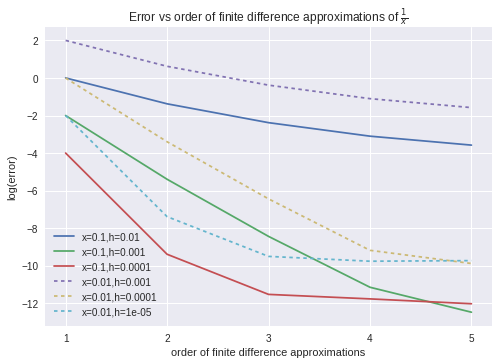
\includegraphics[width=\textwidth]{images/1_x_error_vs_order.png}
      % \caption{This plot show error of using finite difference to approximate the derivative of $\frac{1}{x}$ vs the order of the approximation.}
      % \label{fig:1/x_error_vs_order}
      \index{figures}
    \end{figure}
  \end{columns}

\end{frame}

\begin{frame}
  \frametitle{Stencil used}
  \begin{columns}
    \column{0.3\textwidth}
    Some explanation This is just to check the extent
    \column{0.7\textwidth}
    \begin{figure}[hbt!]
      \centering
      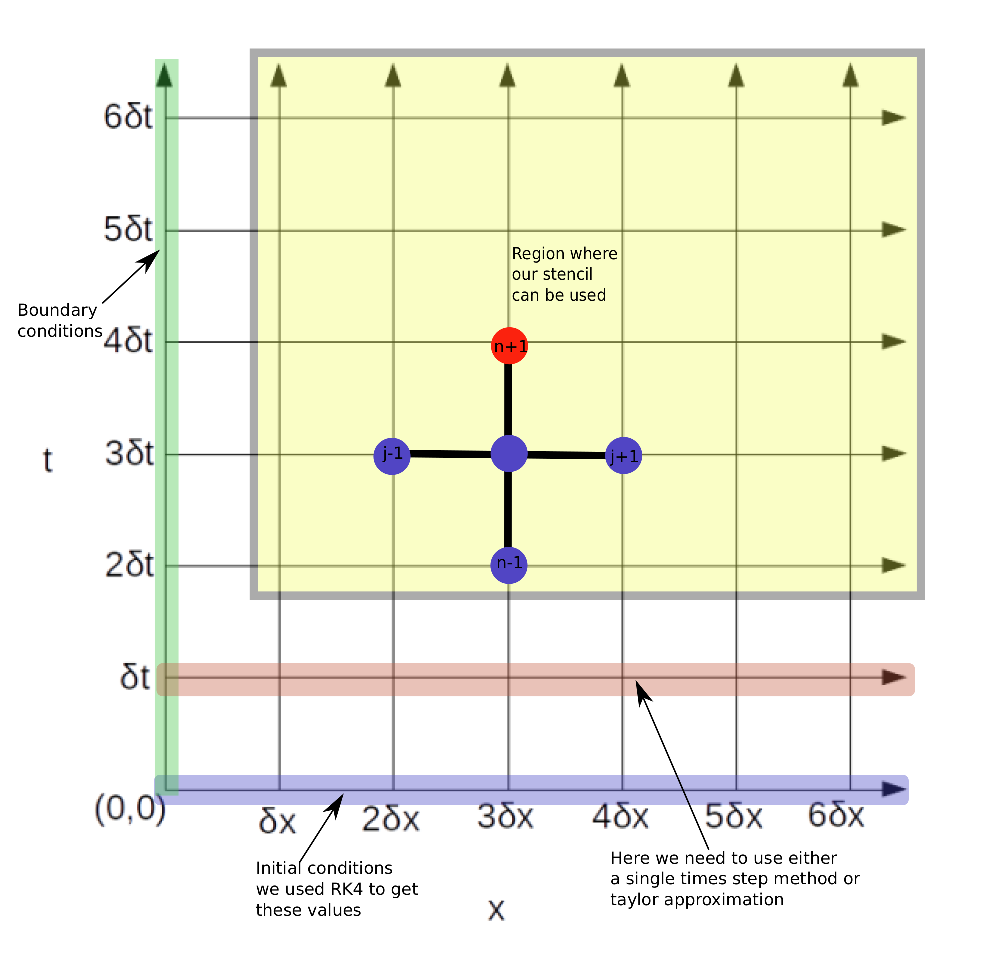
\includegraphics[width=.75\textwidth]{images/labelled_grid.eps}
      % \caption[Stencil used and the computational grid]{This figure shows our computational domain and the stencil used. To calculate the value at any point on the grid we need the red dot of the stencil to be at that grid point, observe that we can not put the red circle of the stencil in the regions that are green, red and blue. \textbf{Yellow}: We can use our stencil in this region. \textbf{Red}: We have to use any other methods or stencils that only depend on the last time step, we used taylor series because it was the easiest to use in our case. \textbf{Blue}: This is the initial configuration of system that we evolve in time, i.e. initial conditions of our system.}
      % \label{fig:grid_with_stencil_and_regions}
      % \index{figures}
      % \end{figure}
    \end{figure}
  \end{columns}

\end{frame}

\begin{frame}
  \frametitle{Profiles used}

\end{frame}

\begin{frame}
  \frametitle{Results}

  \begin{equation*}
    \psi(t=0, x)=A \exp \left(\frac{-\left(x-x_{0}\right)^{2}}{\delta^{2}}\right)
  \end{equation*}

  \begin{columns}
    \column{0.5\textwidth}
    \begin{figure}
      \centering
      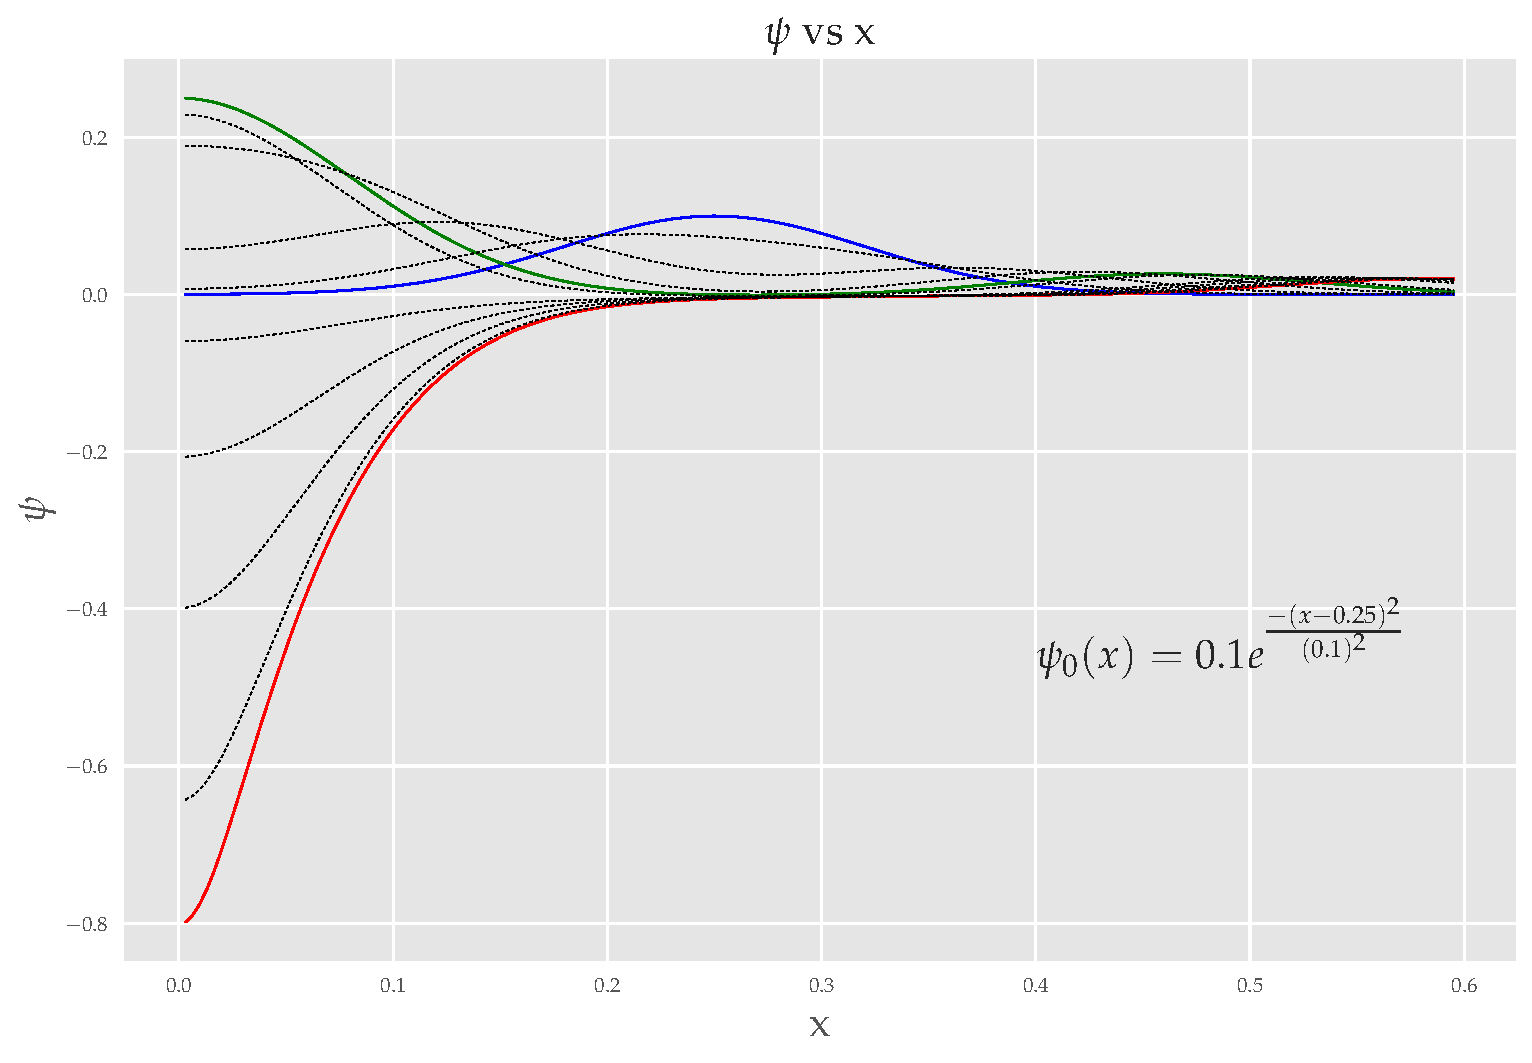
\includegraphics[width=1\linewidth]{images/super_Gaussian.pdf}
    \end{figure}
    \column{0.5\textwidth}
    \begin{figure}
      \centering
      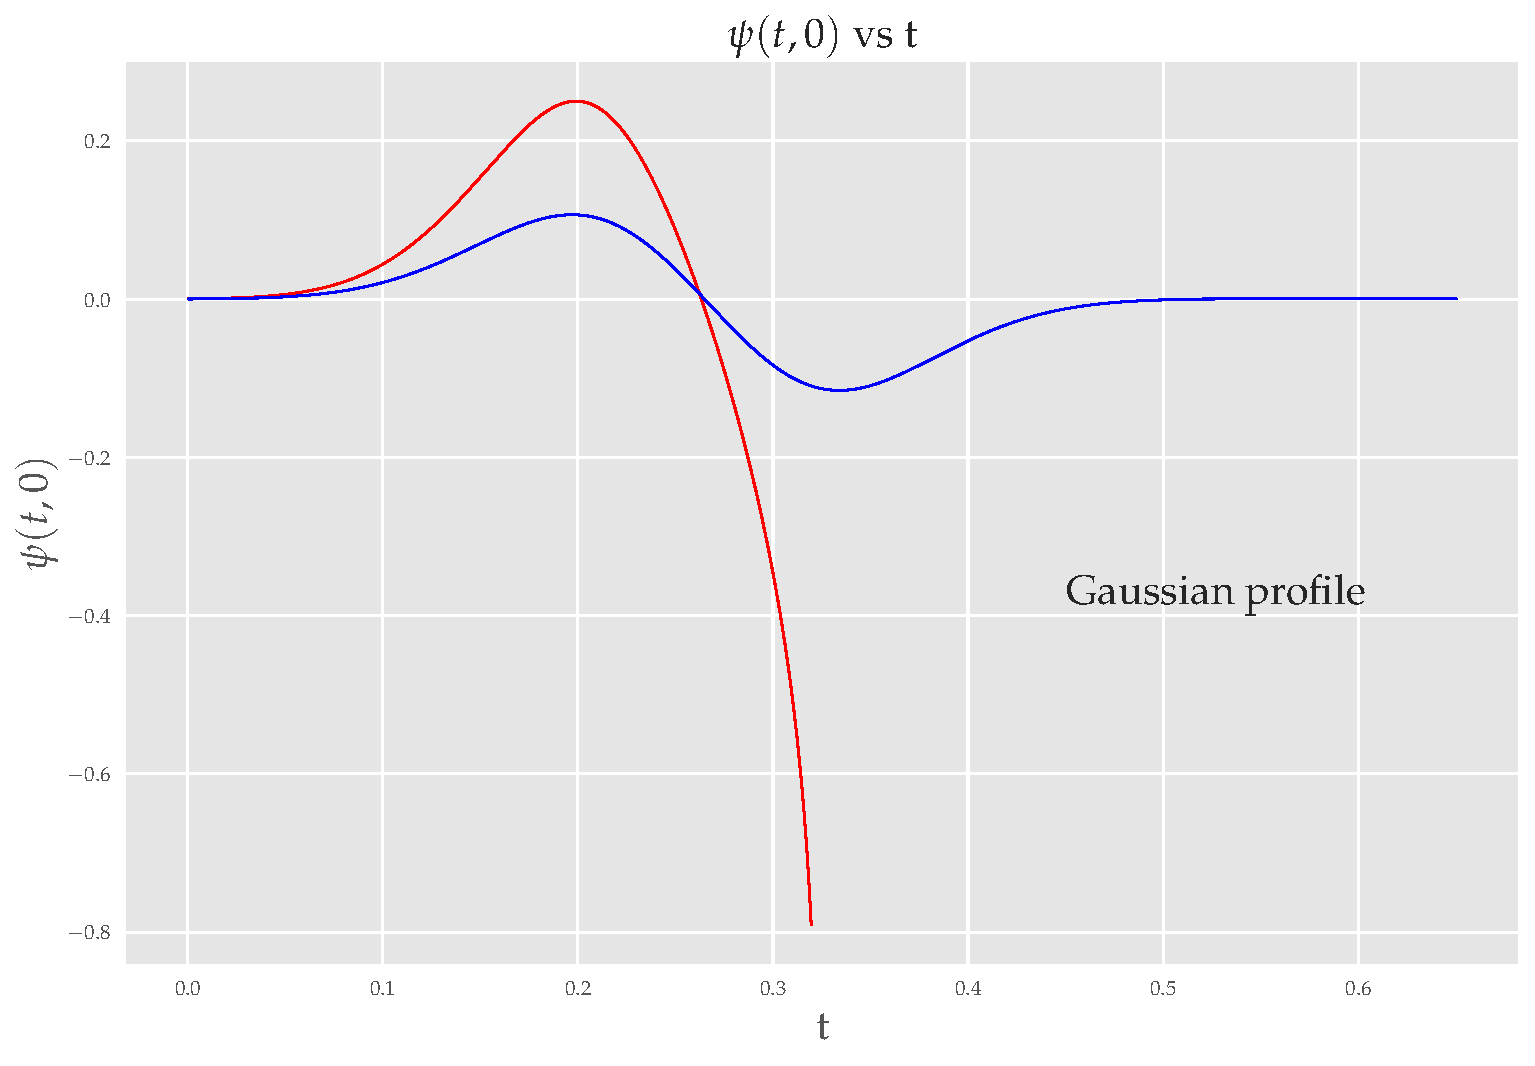
\includegraphics[width=1\linewidth]{images/at0_Gaussian.pdf}
    \end{figure}
  \end{columns}

\end{frame}

\begin{frame}
  \frametitle{Results}

  \begin{equation*}
    \psi(t=0, x)=A x^{2} \exp \left(\frac{-\left(x-x_{0}\right)^{2}}{\delta^{2}}\right)
  \end{equation*}

  \begin{columns}
    \column{0.5\textwidth}
    \begin{figure}
      \centering
      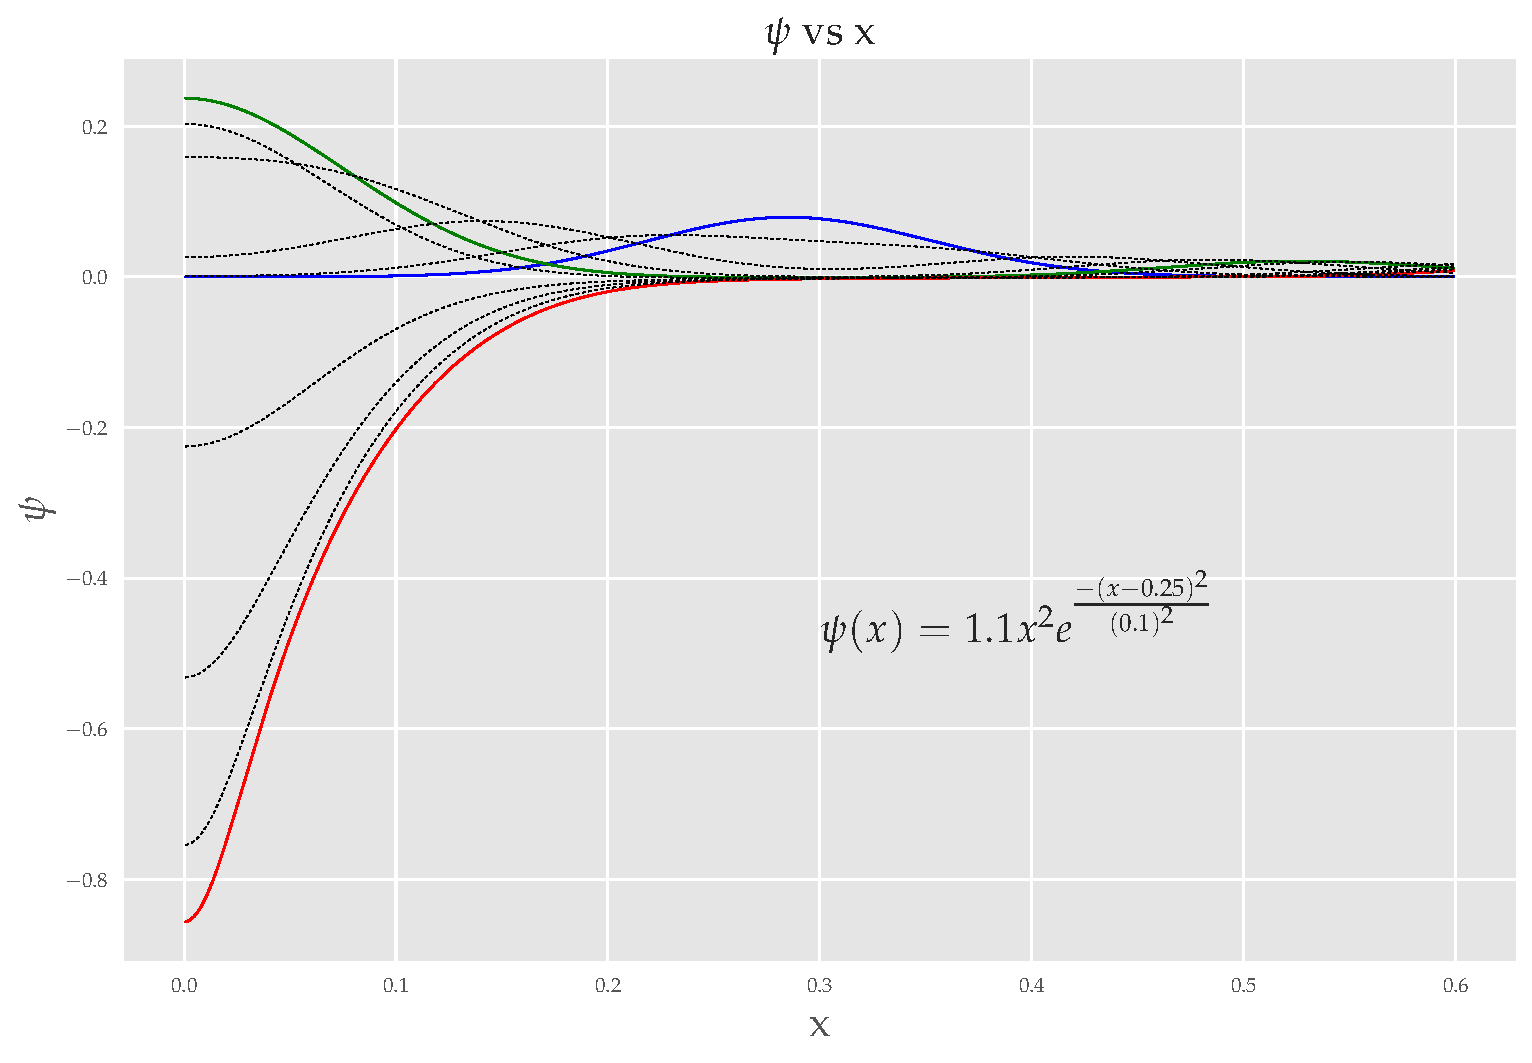
\includegraphics[width=1\linewidth]{images/super_mod.pdf}
    \end{figure}
    \column{0.5\textwidth}
    \begin{figure}
      \centering
      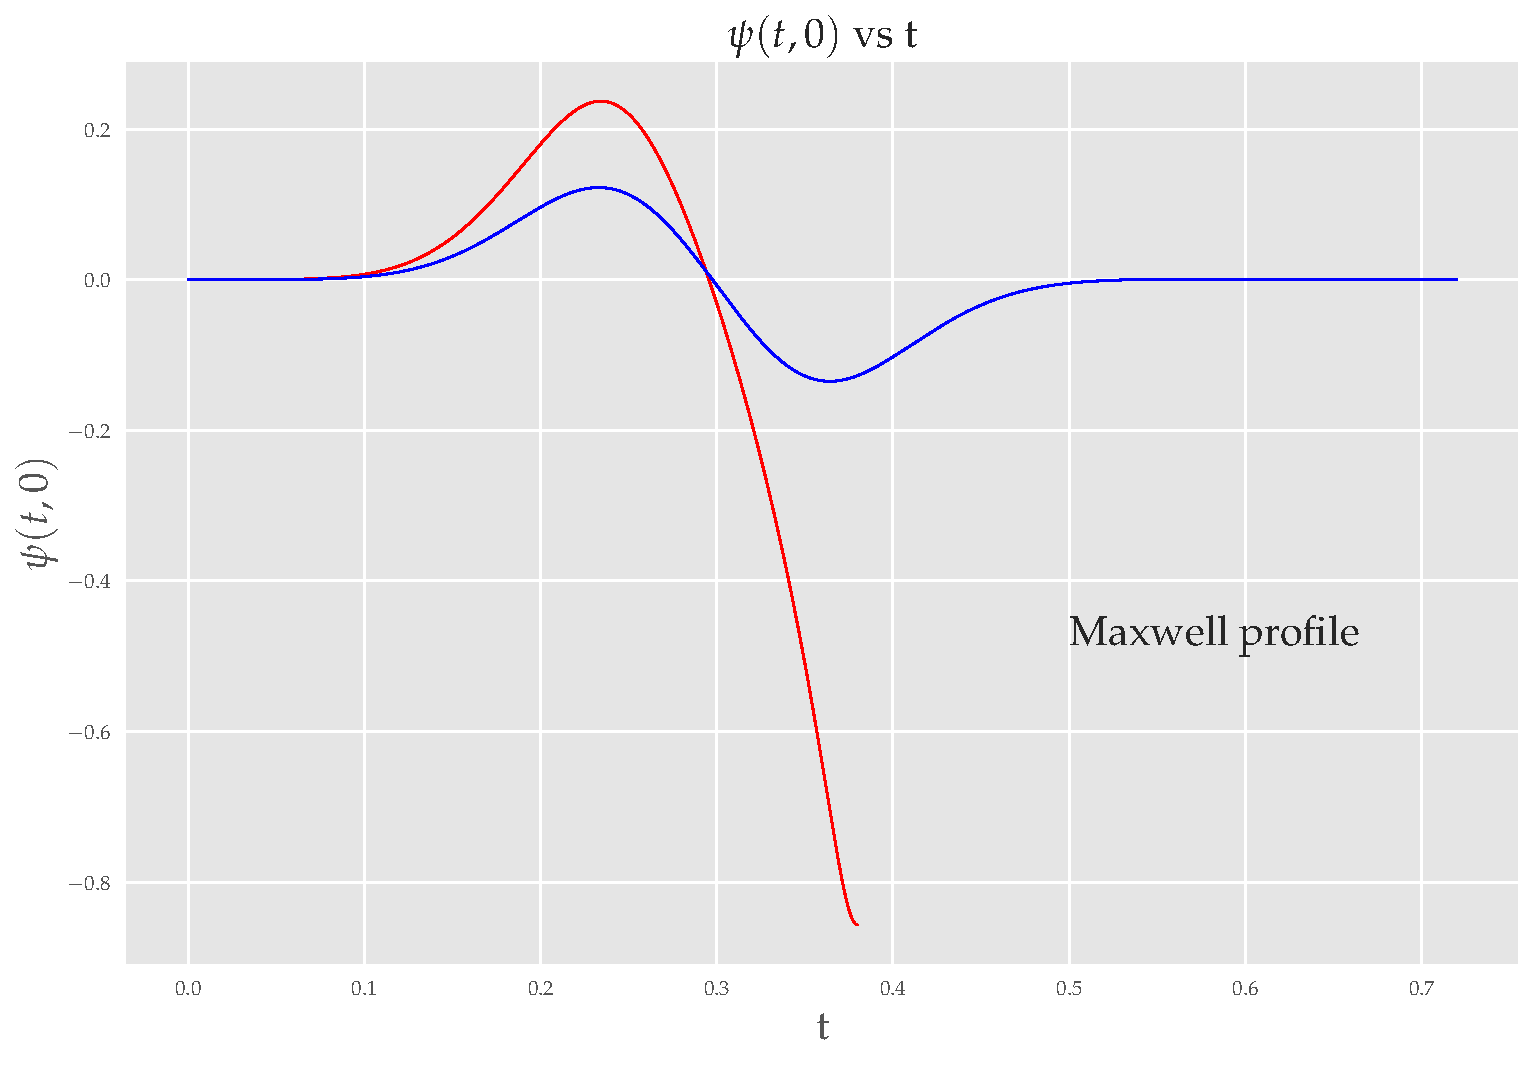
\includegraphics[width=1\linewidth]{images/at0_mod.pdf}
    \end{figure}
  \end{columns}

\end{frame}

\begin{frame}
  \frametitle{Results}

  \begin{equation*}
    \psi(t=0, x)=A\left(\tanh \left(\frac{-\left(x-x_{0}\right)}{\delta^{2}}\right)+1\right)
  \end{equation*}

  \begin{columns}
    \column{0.5\textwidth}
    \begin{figure}
      \centering
      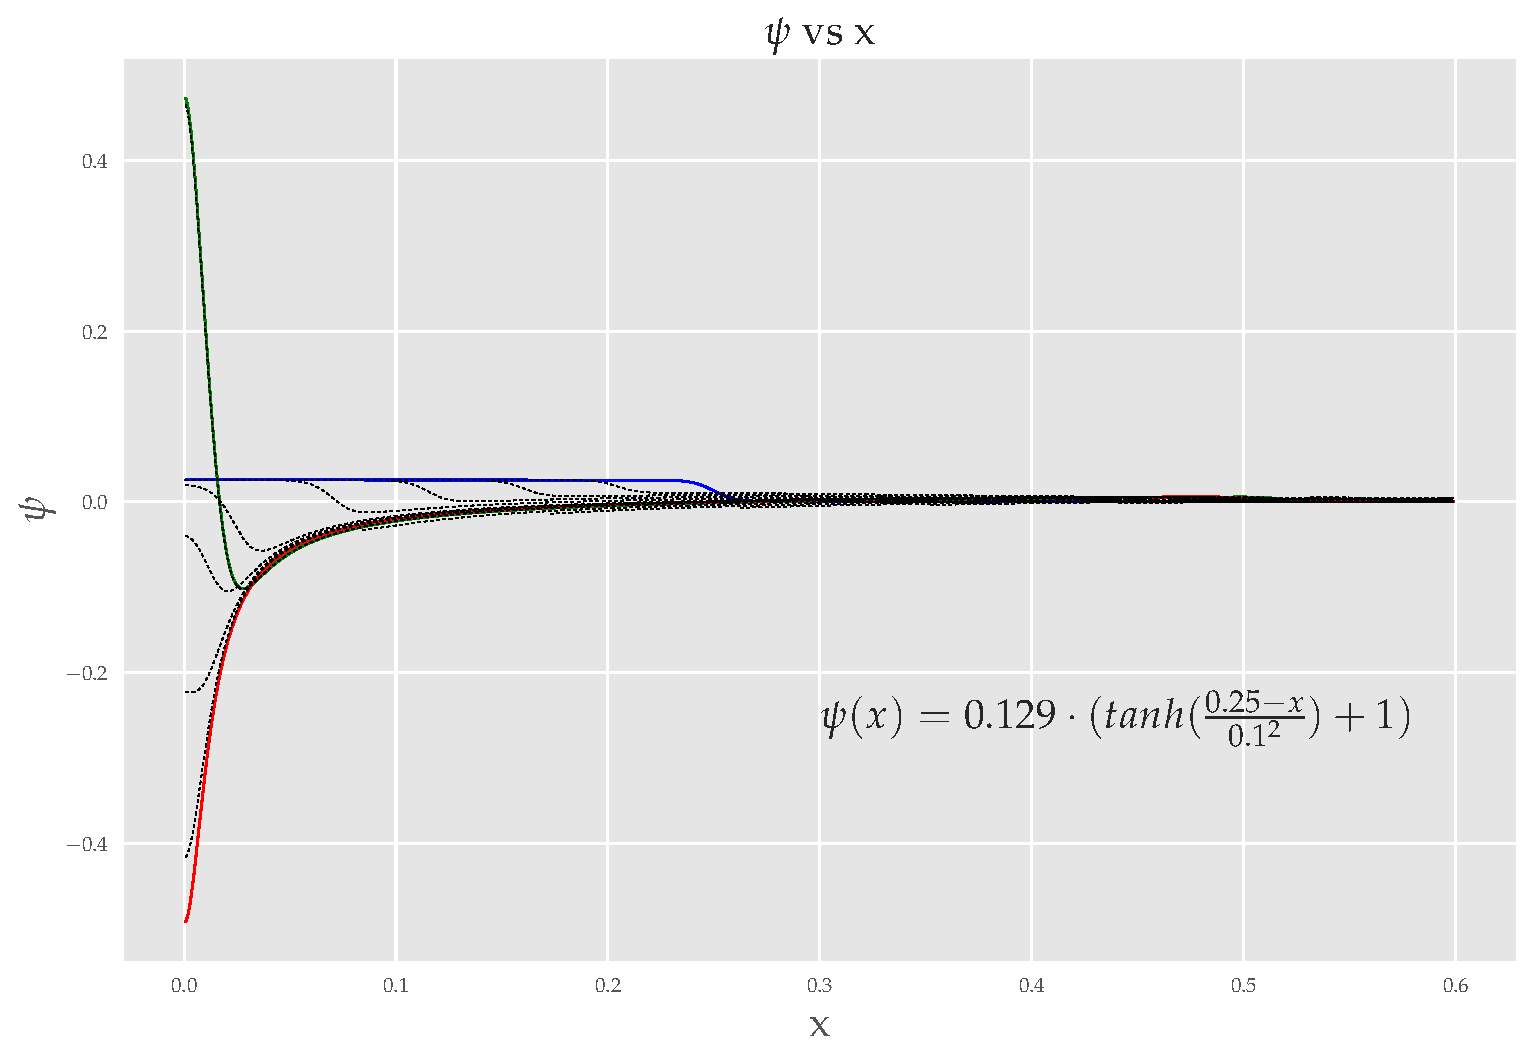
\includegraphics[width=1\linewidth]{images/super_tanh.pdf}
    \end{figure}
    \column{0.5\textwidth}
    \begin{figure}
      \centering
      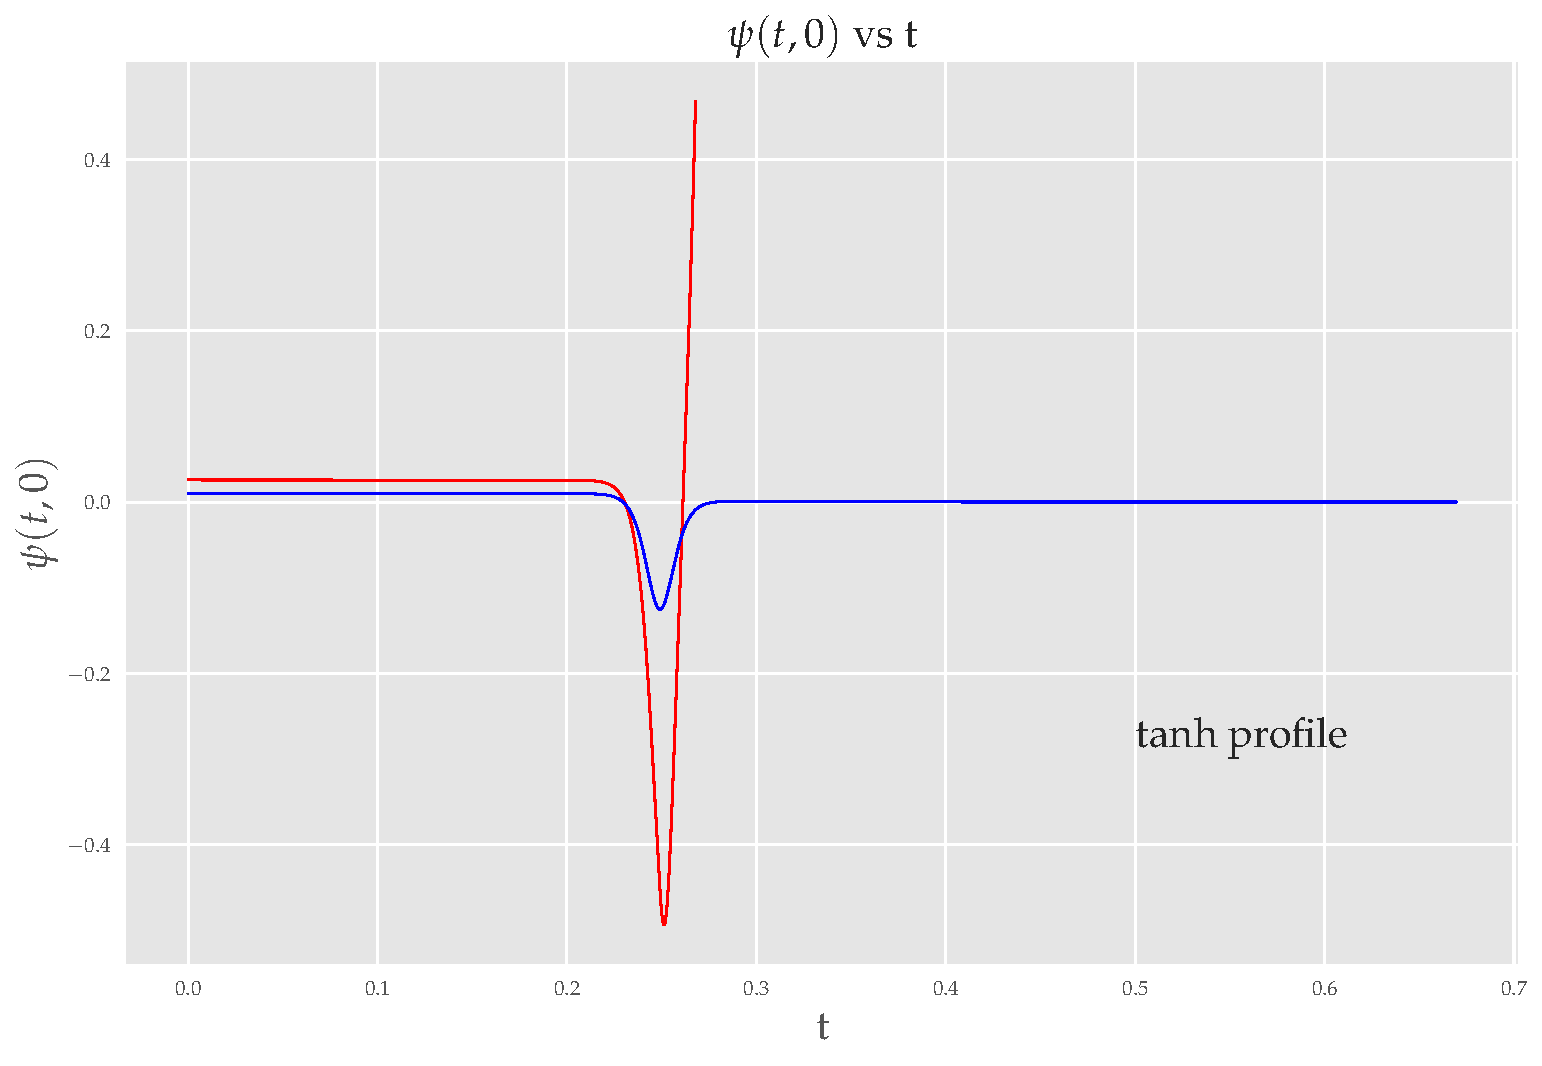
\includegraphics[width=1\linewidth]{images/at0_tanh.pdf}
    \end{figure}
  \end{columns}

\end{frame}

\begin{frame}
  \frametitle{Results}

  \begin{equation*}
    \psi(t=0, x)=A\left(\tanh \left(\frac{-\left(x-x_{0}\right)}{\delta^{2}}\right)+\tanh \left(\frac{\left(x-x_{0}+w\right)}{\delta^{2}}\right)\right)
  \end{equation*}

  \begin{columns}
    \column{0.5\textwidth}
    \begin{figure}
      \centering
      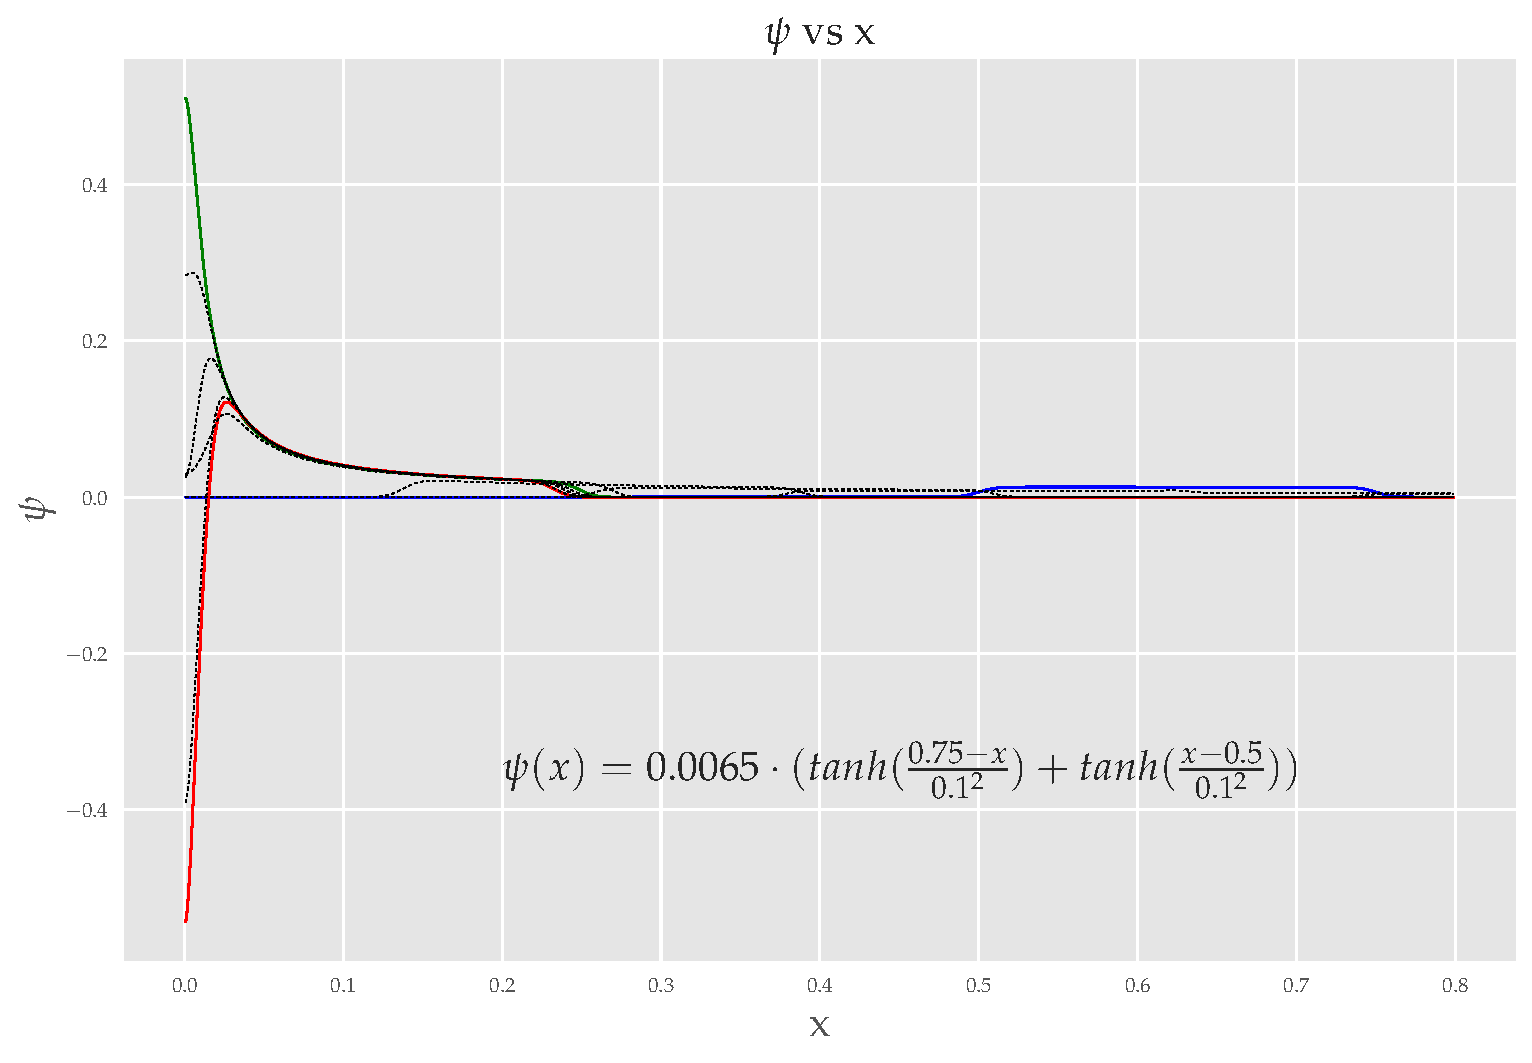
\includegraphics[width=1\linewidth]{images/super_shell.pdf}
    \end{figure}
    \column{0.5\textwidth}
    \begin{figure}
      \centering
      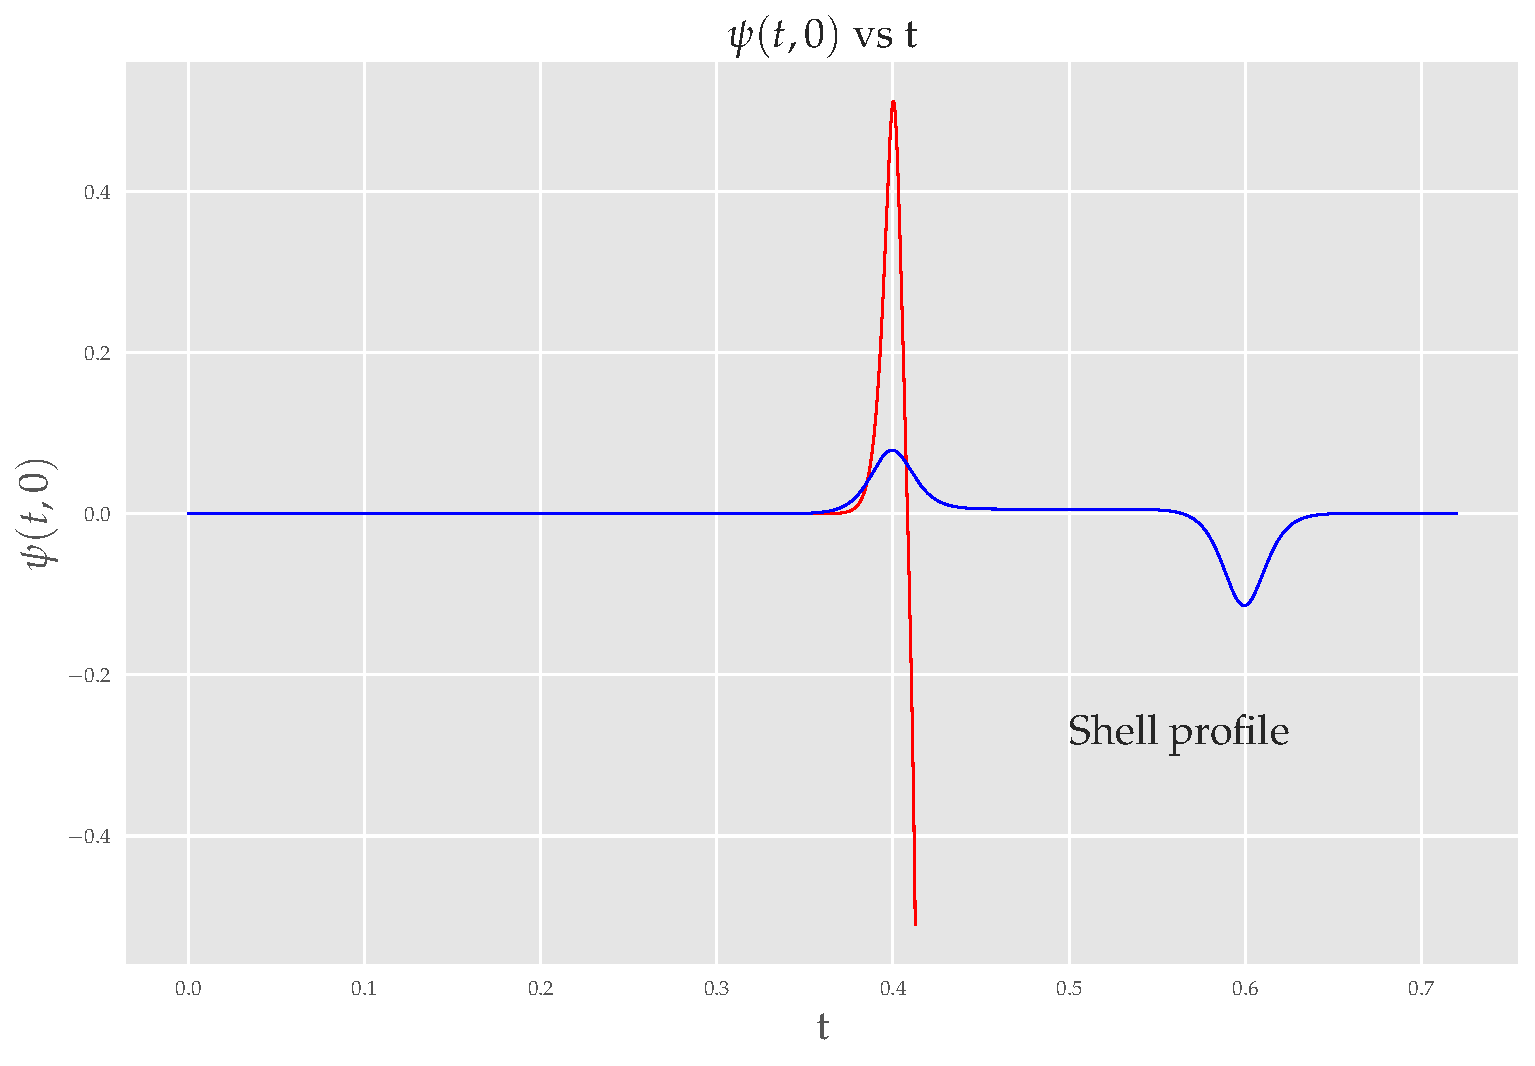
\includegraphics[width=1\linewidth]{images/at0_shell.pdf}
    \end{figure}
  \end{columns}

\end{frame}


\begin{frame}
  \frametitle{Conclusion}

\end{frame}


\begin{frame}
  \frametitle{}
  Thank you!
\end{frame}

%---------------------------------------------------------


%---------------------------------------------------------
% \begin{frame}  % Example of the \pause command
%   This slide is to test mathematical formulas \pause

%   $$E=mc^2$$ \pause

%   as well as the ``pause'' functionality
% \end{frame}
%---------------------------------------------------------

% \section{Caltech student pranks}

% %---------------------------------------------------------
% %Highlighting text
% \begin{frame}
%   \frametitle{Gravitational Collapse}

%   This is a brief introduction of \alert{Caltech pranks}.

%   \begin{block}{Definition}
%     Prank: a practical joke or mischievous act
%   \end{block}

%   \begin{alertblock}{Axiom}
%     Caltech pranks are a key part of the institute's history and identity.
%   \end{alertblock}

%   \begin{examples}
%     See the next slide for a prank example.
%   \end{examples}
% \end{frame}
% %---------------------------------------------------------


% %---------------------------------------------------------
% %Two columns
% \begin{frame}
%   \frametitle{Hollywood sign}

%   \begin{columns}

%     \column{0.45\textwidth}

%     \begin{figure}
%       \centering
%       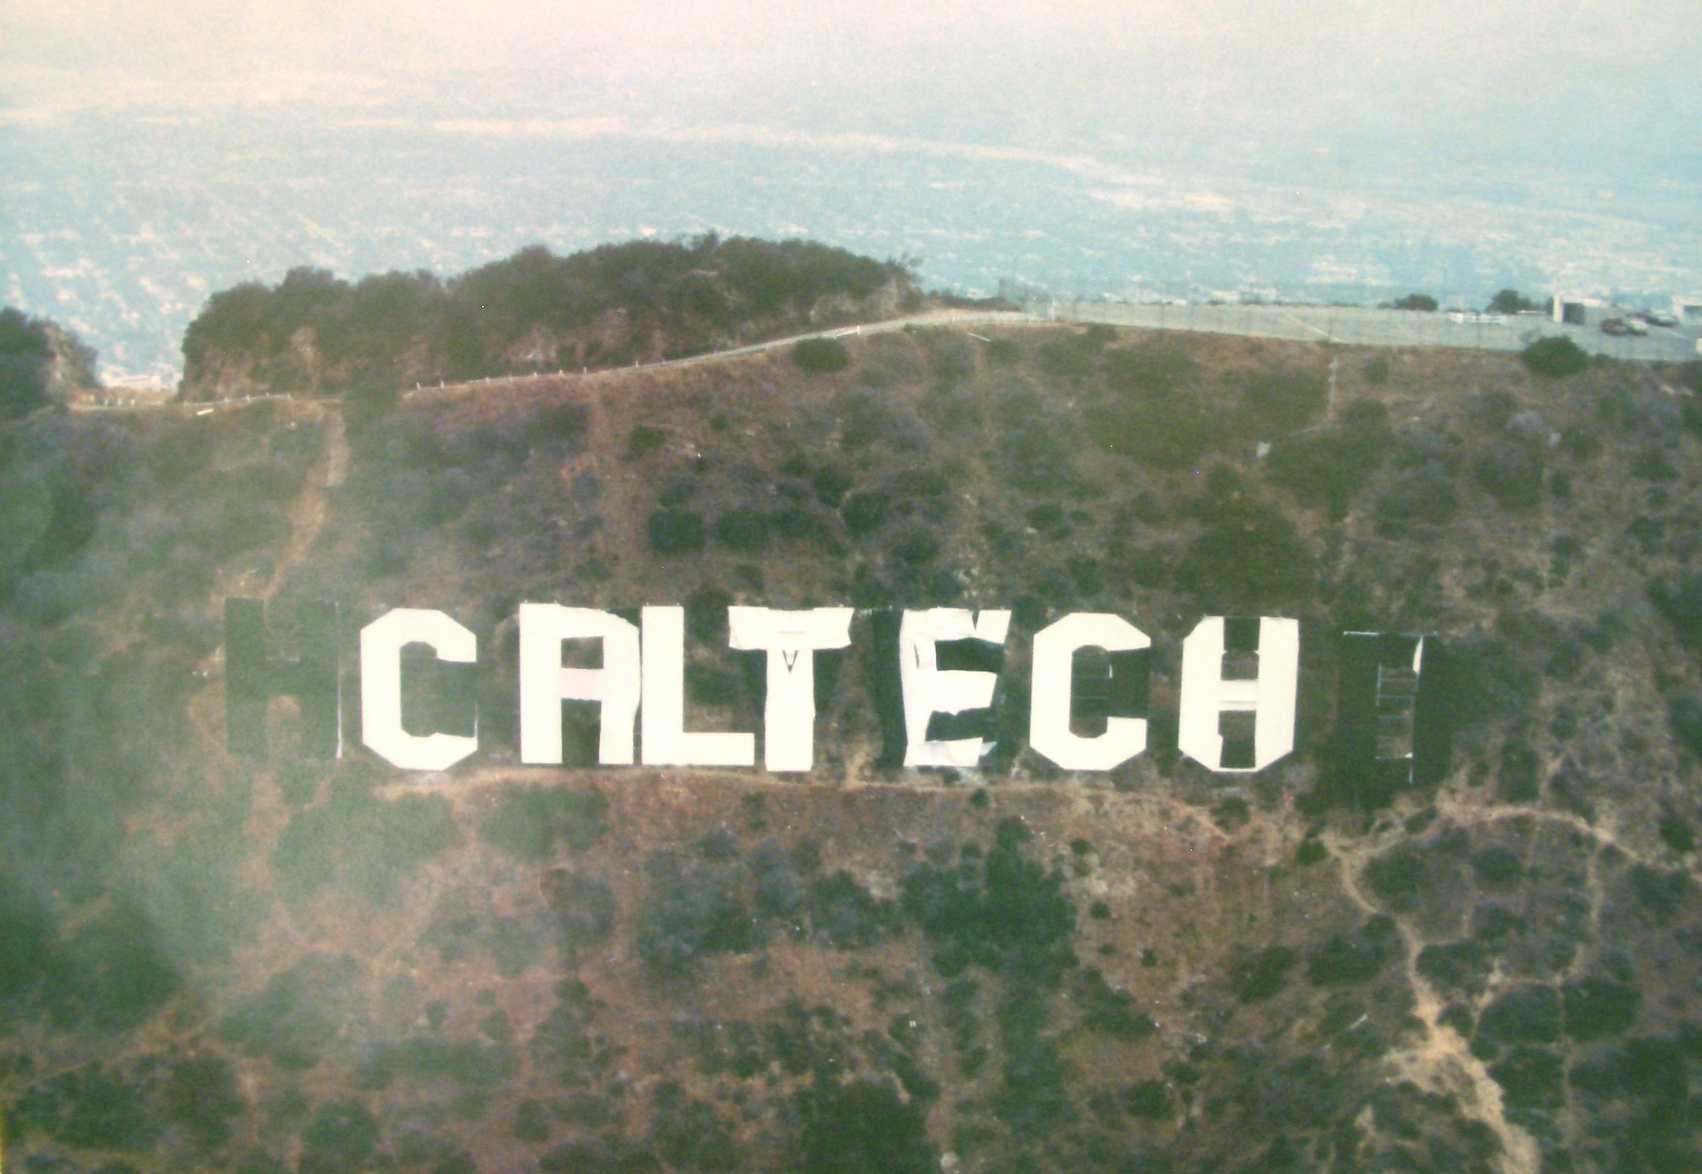
\includegraphics[width=\columnwidth]{./figures/hollywood_caltech.jpg}
%       \caption{``Hollywood is still mad about that,'' says Autumn Looijen, author of \emph{Legends of Caltech III: Techer In the Dark.} \tiny{(Photo downloaded from: http://brennen.caltech.edu/autobiography/automaster2.htm)}}
%       \label{fig:hollywood_prank}
%     \end{figure}


%     \column{0.55\textwidth}
%     In May 1987, undergraduates from Page and Ricketts houses combined forces (and several hundred dollars) to purchase enough black and white plastic, transformed the Hollywood sign to read ``Caltech''.

%     \small{(Reference: http://www.admissions.caltech.edu/pranks)}

%   \end{columns}
% \end{frame}
%---------------------------------------------------------


\end{document}